\documentclass{article}
\usepackage{algorithm}
\usepackage{algpseudocode}
\usepackage{geometry}
\usepackage{xcolor}
\usepackage{graphicx}
\usepackage{mathtools}
\usepackage{enumitem}
\usepackage{amsmath,amsthm}
\usepackage[english]{babel}
\usepackage{amsfonts}
\usepackage{thmtools}
\usepackage{fancyhdr}
\graphicspath{{./IMG/}}
\usepackage{color}   %May be necessary if you want to color links
\usepackage{hyperref}
\hypersetup{
    colorlinks=true, %set true if you want colored links
    linktoc=all,     %set to all if you want both sections and subsections linked
    linkcolor=blue,  %choose some color if you want links to stand out
}

%-------------- HEADER -- FOOTER --------------------------------------------------------
% Main Title
\newcommand{\PaperTitle}{MATH 327 Build Your Own Assesment}
% Sub Title
\newcommand{\PaperSubTitle}{Write-up} 
% Authors
\newcommand{\Authors}{Aiden Taylor(30092686) and Noah Pinel(30159409)}

% Title Page
\title{
    % \vspace{2in}
    \textmd{\textbf{\PaperTitle\\ \PaperSubTitle}}\\
    \author{Created by \Authors}
    \date{}
    \vspace{6in}
}

%--- LAZY -----------------------------------------------------------------------------------
\newcommand{\R}{\mathbb{R}}
\newcommand{\Z}{\mathbb{Z}}
\newcommand{\ps}{\{p_n\}}



%---------------------HEADER FOOTER-----------------------------------------------------------
\pagestyle{fancy}
\fancyhead{}

\fancyhead[L]{\slshape\nouppercase{\leftmark}}
\rhead{MATH 327 - BYOA Write-up}
\fancyfoot{}
 
% Hide section for format purposes i.e ToC and Abstract.
\newcommand\invisiblesection[1]{%
  \refstepcounter{section}%
  \addcontentsline{toc}{section}{\protect\numberline{\thesection}#1}%
  \sectionmark{#1}}

%----------------START-------------------------------------
\begin{document}
\maketitle % Print the title
\thispagestyle{empty}
\newpage
\fancyfoot[R]{\thepage}
%----------------ABSTRACT---------------------------------------------------
\invisiblesection{Abstract}
\begin{abstract}
  This file contains the written portion of our assignment, we briefly introduce each piece of code we wrote, 
  the subject, and how it relates to the course content. Alongside this write-up there will be the source 
  code for each of our respected programs and a short video demonstrating their functionality.

  Cheers, 
  Aiden.T and Noah.P
\end{abstract}
\newpage
%----------------TABLE OF CONTENTS------------------------------------------
\tableofcontents
\invisiblesection{Table of contents}
\newpage

% -------- NOAH WU #1/2 --------
\section{Implementation of The Sieve of Eratosthenes in Python}
\subsection{Overview}
The Sieve of Eratosthenes is a type of prime sieve. Prime sieves are algorithms 
that are very good at generating prime numbers up to some upper bound n, where $n\in\Z^+$.
The following sections explain the Implementation process of simulating the Sieve of Eratosthenes 
in the programming language Python.

\subsection{The Implementation}
My first run in with the sieve of Eratosthenes was during my number theory course, the 
mechanical nature of the sieve seemed to be a perfect way to utilize a computer to do
some interesting math. The entirety of the program relies on the algorithm below, so here 
are the meat and potatoes of the whole thing,
\begin{algorithm}
  \caption{: An algorithm for The Sieve of Eratosthenes}
  \begin{algorithmic}[1]
  \Require: $n > 0$
  \Ensure: List of prime numbers 2, ..., n
  \State Sieve$(n):$
      \State Populate a boolean list P size 2, ..., n.
      \State Initialize all index values to True.
      \For{$i = 2,..., n+1$:} 
          \State if P[i] TRUE
          \For{$j = i^2, i^2+1, i^2+3,..., n$:}
            \State set P$[j]$ False
          \EndFor
      \EndFor
    \State Return P
  \end{algorithmic}
\end{algorithm}\\
Simply put, we have a list of size $2,..., n$. We set all values of our list to True, then starting at 2 we loop through each index
setting multiples of the respected current position to false. After this has run, we are left with a list where all prime values are
unchecked, that is, they remain True while composite numbers are false. Below is a visual of the algorithm working for a list of size 10.
\begin{center}
  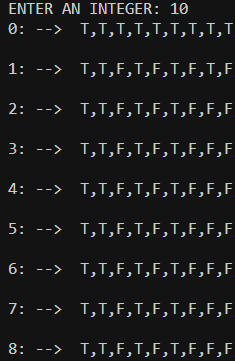
\includegraphics[scale=0.4]{Sieveiter.png}
\end{center}
We can see that after 8 iterations of following the algorithm the only index values set True are $2,3,5,7$, i.e., the first 4 primes. 
Now as cool as it is to visualize the algorithm I feel like finding the number of primes $\leq$ some large n is a lot more interesting.
To help with run time I disabled the visual aspect of the algorithm and was able to find a value for the primes up to $100,000,000$.
\begin{center}
  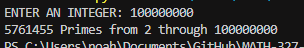
\includegraphics[scale=1.0]{primesFound.png}
\end{center}
Using the forbidden site Wolfram Alpha to verify, there are indeed 5,761,455 primes in between 2 and 100,000,000.
\subsection{Conclusion}
The last calculation presented took just about an epsilon under a minute to calculate, which for an algorithm that has been around for thousands of years
I feel is very impressive, thus, Eratosthenes sieve is a powerful tool to find primes up to some appropriate positive integer. This problem also displays the interplay between Mathematics 
and Computer Science and how they complement each other very well. The source code for Sieve.py will be included in our submission with documentation if you're
wanting to poke around.

\newpage
% -------- NOAH WU #2/2 --------
\section{Visual Representation of Euler's Phi Function in Python}
\subsection{Overview}
Euler is one of the most well known Mathematicians ever, the following program I implemented 
is a visual representation of a function he created, namely the Euler Phi function.
\subsection{What is it?}
Euler's Phi function takes in a positive value n, and counts the number of relatively prime numbers up to the original n.
For example $\Phi(10)= |\{1,3,7,9\}| = 4$, so Euler's function is telling us that from 1-10, there are 4 numbers coprime to 10.

\subsection{The Implementation}
While reading the MATH-327's assigned text book I really enjoyed seeing all the visual representations of the math we were learning. 
I decided to use python to create a visual of this special function. The process of coding this wasn't too bad, it consisted of reading in
an n value, then for each i up to n, I would call the Phi function that I wrote, it would simply just check for a $\gcd(i_j, n) == 1$ and if 
it returned true it was added to a list. After I had this list of all 1,..., n's respected Phi function values I was able to use the python library
Matplotlib.pyplot to graph this list against the corresponding n value, figure(\ref{fig:PhiPlot}) is the awesome visual that was generated.\\
\begin{figure}
  \centering
  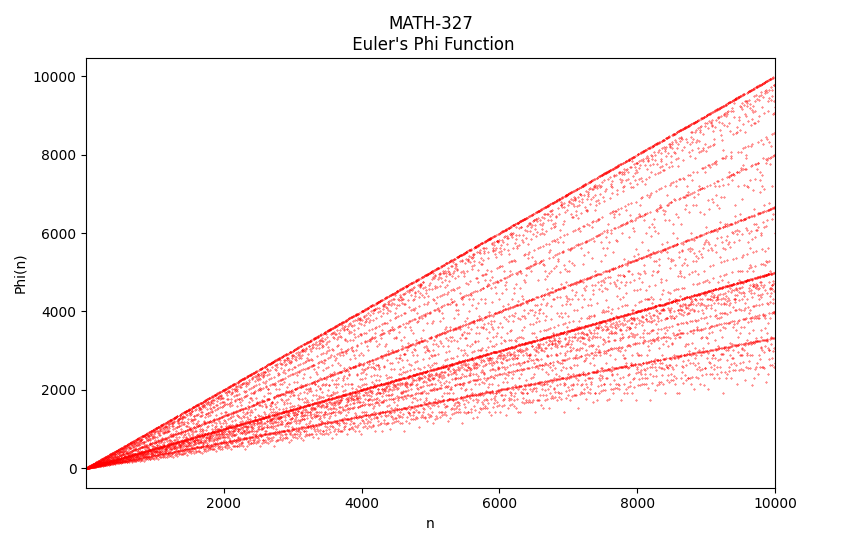
\includegraphics[scale=.4]{PHI.png}
  \caption{Euler's Phi function plotted up to 10,000}
  \label{fig:PhiPlot}
\end{figure}
\subsection{Conclusion}
The visual representations that arise from ideas in number theory are amazing to look at, and Euler's Phi function is no excuse. The power computers 
give us to generate these models is just another example of how technology can give us deep insight into mathematical concepts.

% Aiden Writeup 1/2
\section{Implementation of a 2-Variable LDE Solver in C}
\subsection{Overview}
The definition from Weissman's Illustrated Theory of Numbers says, ``A Diophantine Equation is an equation
involving integers, variables, and the elementary operations of addition and substraction. Diophantine equations
are linear if variables are never multiplied with variables." This program simply solves two variable Linear
Diophantine Equations (LDE's) provided by the user.
\subsection{The Implementation}
We learned this semester that to solve LDE's we need to use the Extended Euclidean Algorithm (EEA) to find a base
solution that itself is used to find the general solution to the LDE in question. With that in mind,
my implementation of the EEA by Tabular Method is as follows,
\renewcommand{\algorithmicrequire}{\textbf{Input:}}
\begin{algorithm}
\caption{: An algorithm for the EEA by Tabular Method}
\begin{algorithmic}[1]
\Require{ $a,b$} \Comment{Coefficients of the two variables of the LDE}
	\State{$a1 \leftarrow a$} \Comment{Placeholder variables for calculating remainder}
	\State{$b1 \leftarrow b$}
	\State{$i=j \leftarrow 1$} \Comment{Placeholder variables for EEA table calculations}
	\State{$k= \ell = temp\_\ell = temp\_j \leftarrow 0$}
	\State{$r = prev\_r = q \leftarrow 0$} \Comment{Remainder, Previous Remainder, and Quotient for GCD calculation}
	\While{true}
		\State{$prev\_r \leftarrow r$}
		\State{$r \leftarrow a1\!\mod{b1}$} \Comment{Calculating remainder}
		\If{$r = 0$}
			\State{break out of loop}
		\EndIf
		\State{$q \leftarrow (a1 - r)/b1$} \Comment{Calculating quotient for division with remainder}
		\State{$a1 \leftarrow b1$}
		\State{$b1 \leftarrow r$}
		\State{$temp\_\ell \leftarrow \ell$}
		\State{$temp\_j \leftarrow j$}
		\State{$\ell \leftarrow i - (q * \ell)$}
		\State{$j \leftarrow k - (q * j)$}
		\State{$i \leftarrow temp\_\ell$}
		\State{$k \leftarrow temp\_j$}
	\EndWhile
	\State{Return $\ell,j$} \Comment{Values to use in base solution for LDE}
\end{algorithmic}
\end{algorithm} \\
\newpage
\noindent In the above algorithm $i,j,k,$ and $\ell$ are the integers representing
\begin{table}[h]
\begin{center}
\begin{tabular}{c|c|c|c}
\textbf{$a$} & \textbf{$b$} & 1 & Row\\
\hline
$i = 1$ & $k = 0$ & $a1 = a$ & $R_1$\\
$\ell = 0$ & $j = 1$ & $b1 = b$ & $R_2$\\
... & ... & ... & ... \\
\end{tabular}
\end{center}
\end{table}

\noindent which are used to represent the table values for the EEA by Tabular Method.
After the base solution has been
computed by the EEA we need to do some simple sign management as the solution from the EEA may
not always be as desired. Then, with the correct base solution, we can calculate the general solution using
\textbf{Corollary 1.25} from the text, or state that there are no solutions if $c$ is not a multiple of $GCD(a,b)$,
from $ax + by = c$.
\begin{center}
  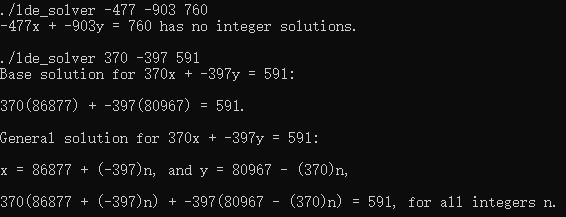
\includegraphics[scale=0.9]{example.PNG}
\end{center}
\subsection{Conclusion}
This was a very interesting program to implement, where most of my time actually went into dealing with
the weird sign
behaviour generated by the EEA, which was a little annoying.
Also, I should probably improve my variable naming as I understand using $i,j,k,$ and $\ell$
most likely makes absolutely no sense to people reading the code for the first time... I'll work on it. 
In the end, I did not test the runtime of my implementation,
but hopefully my use of C can mask the fact that I don't how to optimize code.
\newpage

% Aiden Writeup 2/2
\section{Implementation of the Miller-Rabin Test in C}
\subsection{Overview}
The Miller-Rabin Test is a probabilistic primality test for all positive odd integers greater than 2.
However, in this implementation, we will only be looking at integers between 2 and 2,047 so that we can use the
witness prime 2 to give us precise results (and so that the exponential calculations are not super huge).
\subsection{The Implementation}
For this implementation I took inspiration from the pseudo-code at 
https://en.wikipedia.org/wiki/Miller-Rabin\_primality\_test, 
which would give a much more in depth explanation of the Miller-Rabin Test. Firstly, the user passes
an odd integer $n$ that is within the specified bound. Then, it is broken down into the equation
$n-1 = 2^s d$, where $s > 0$, $d>0$, and $d$ is odd. The reason we need to factor out powers of 2 from $n-1$
is to check if one of the following two congruence relations hold
\begin{itemize}
\item $2^d \equiv1\!\mod{n},$
\item $2^{2^rd} \equiv-1\!\mod{n}, \text{ for some } 0 \leq r < s,$
\end{itemize}
where these congruence relations follow from Fermat's Little Theorem. If one of these relations holds with
$2 < n < 2,047$ ($n$ odd) then we can say $n$ is prime, where 2 is a witness for the primality of $n$. Otherwise, if
neither of these hold, then $n$ is composite, where $2$ is a witness for the compositeness of $n$.
\begin{center}
  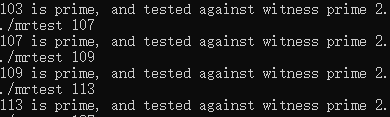
\includegraphics[scale=0.9]{primes.PNG}
  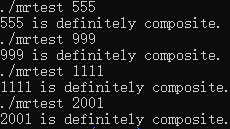
\includegraphics[scale=0.818]{composites.PNG}
\end{center}
\subsection{Conclusion}
Although my implementation only covers a small bound, it is easy to see that by adding more witness primes one could
increase the bound considerably, at the cost of having to deal with huge numbers. I should also mention my use of
geeksforgeeks implementation of a Modular Exponentiation function as dealing with the huge exponential
calculations was definitely the biggest hurdle in this implementation (see the source code for the reference).
In the end, I am pretty happy with this implementation, and I had a lot of fun researching this test and learning
how important probability is in primality tests (even if my implementation didn't use any probability).

\end{document}
